\section{Durchführung}
\label{sec:Durchführung}

\subsection{Aufbau}
\label{sec:Aufbau}

\begin{figure}
    \centering
    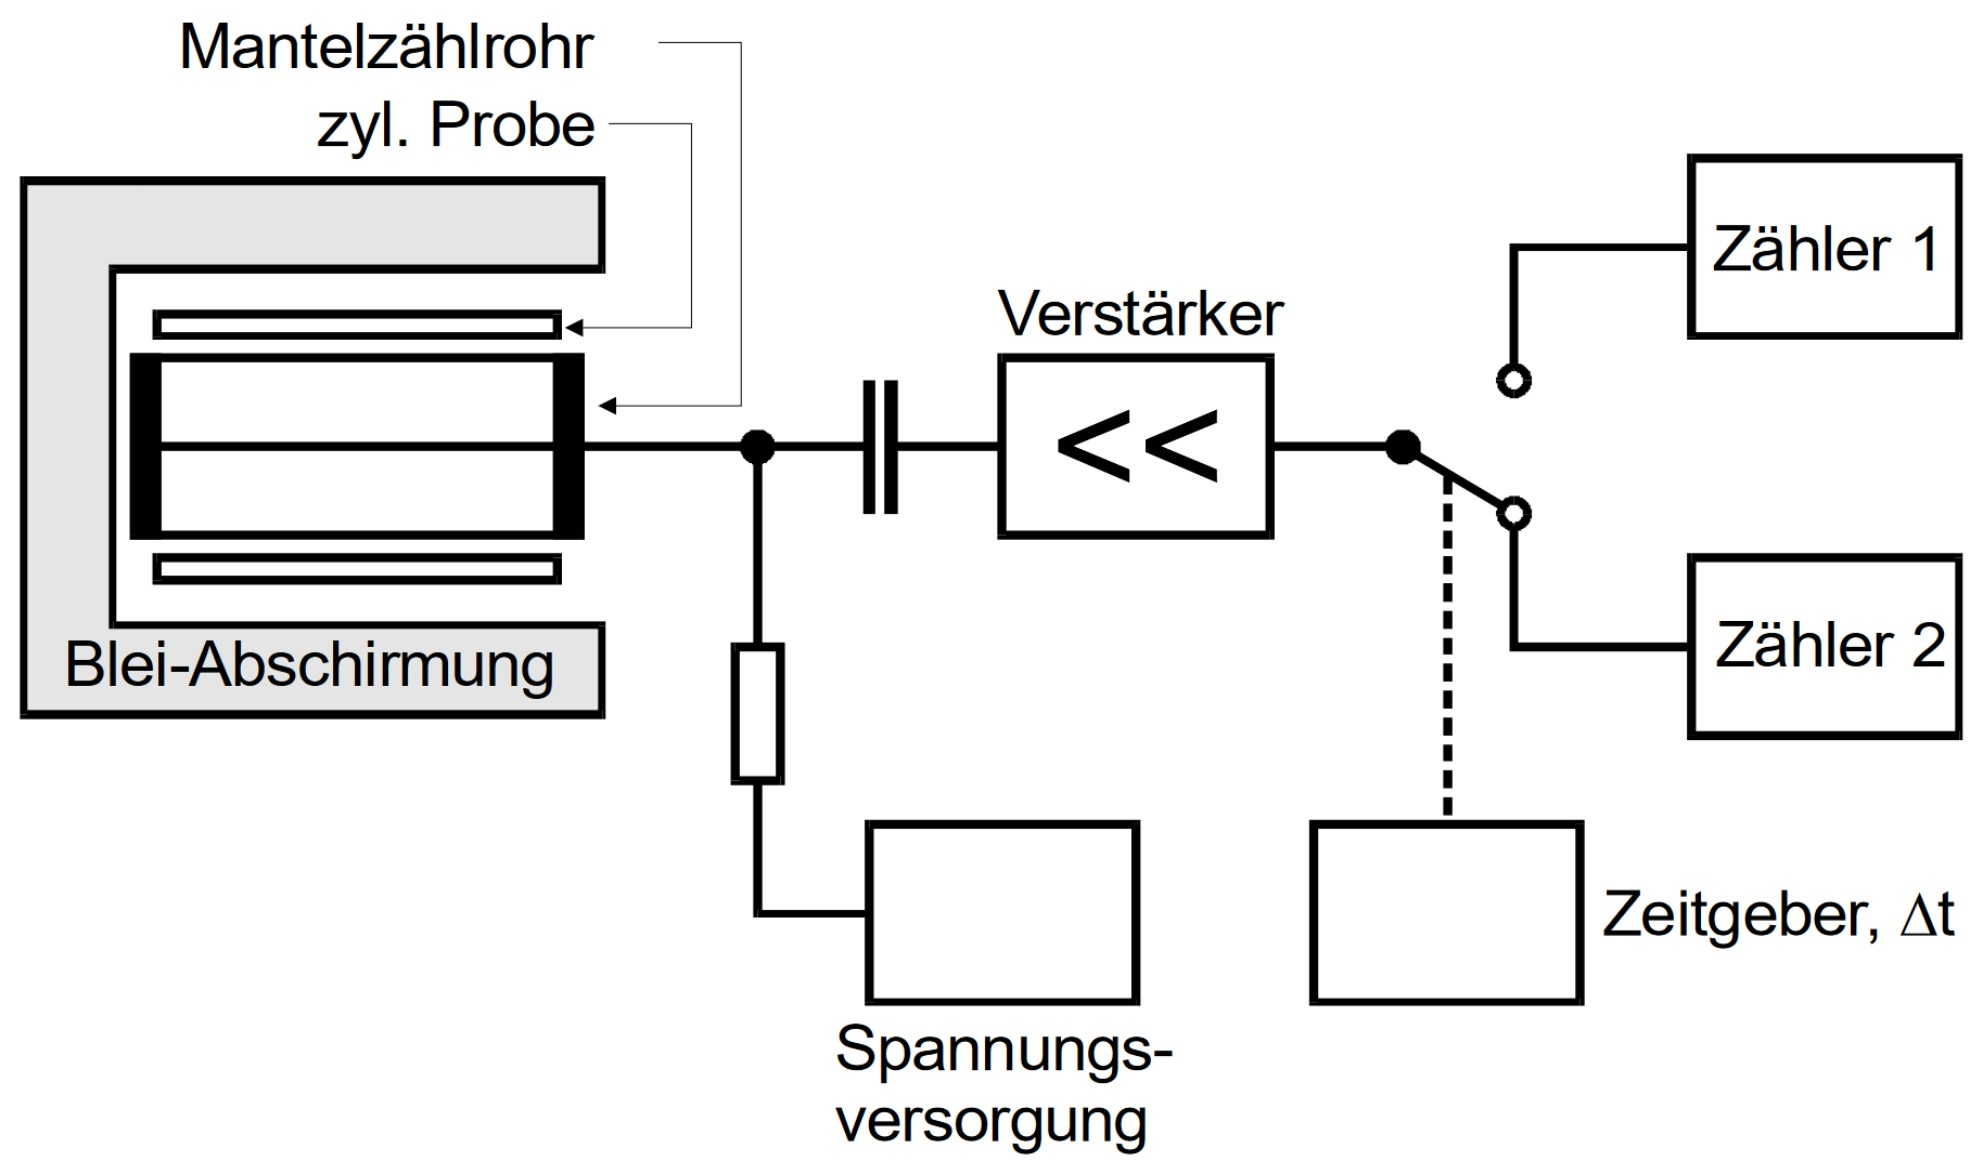
\includegraphics[width=0.8\textwidth]{img/Aufbau.jpg}
    \caption{Schematischer Versuchsaufbau \cite{V702}.}
    \label{fig:Aufbau}
\end{figure}

Der Versuchsaufbau ist in Abbildung \ref{fig:Aufbau} dargestellt.
Er besteht aus einem Geiger-Müller-Zählrohr mit Bleimantel, einem Verstärker, einem Zählwerk mit zwei Zählern und einem Zeitgeber.
Die Impulse des Zählrohrs werden durch den Verstärker verstärkt und an das Zählwerk weitergeleitet.
Das Zählwerk schaltet nach einer einstellbaren Zeit $\Delta t$ zwischen den beiden Zählern um.
Die Isotope werden in einer Quelle für thermische Neutronen platziert.

\subsection{Messung}
\label{sec:Messung}

Zunächst wird die Nullrate $N_0$ gemessen. Der Zeitgeber wird auf $\Delta t = \SI{500}{\second}$ eingestellt und die Anzahl der Impulse $N_0$ gemessen.
Für die Messung von Vanadium wird die Zeit auf $\Delta t = \SI{30}{\second}$, für Silber auf $\Delta t = \SI{10}{\second}$ eingestellt.
Als erstes wird die Zählrate $N_{\text{Ag}}$ von Silber gemessen. Dazu wird die Probe aus der Neutronenquelle genommen und über das Zählrohr gestülpt.
Es werden für sieben Minuten die Impulse gemessen. Anschließend wird die Probe wieder in die Quelle gegeben.
Als nächstes wird die Zählrate $N_{\text{V}}$ von Vanadium gemessen. Dazu wird die Probe aus der Neutronenquelle genommen und über das Zählrohr gestülpt.
Es werden für 15 Minuten die Impulse gemessen. Anschließend wird die Probe wieder in die Quelle gegeben.
Die Messung von Silber wird ein zweites mal durchgeführt.